\subsection{Component Performance}
\label{sec:performance_components}

The only performance parameter considered is processing time, as this determines how long a user must wait on an encryption.
None of the supported constructs use pre-computations or other processing-for-memory (or disk space) trade-offs, so neither
I/O nor memory usage are important.

To measure the processor time spent at various levels, the \emph{Visual Studio Profiler Tools} are used.\footnote{The Visual
Studio Profiler Tools are built-in to Visual Studio, the most common IDE for C\#.} Performing a CPU Sampling with these tools
provide a look into which methods are used, and how often, based on random samples taken while a program is running. A lot of
samples are taken: the program described below ran in \(4.5 \text{ seconds}\) and yielded 806 samples. Looking at the number of samples
that involve a certain function gives an approximation of how often that function is used.\footnote{The full dataset can be
found in Appendix \ref{app:component-performance-data}.}

There are several different abstraction levels to be tested when using OpenECC encryption: on the top-most level there are concepts
such as encryption, decryption, key generation, and curve preparation, on lower levels there are other construct. To profile the time
spent on each concept, a small program was written (see Figure \ref{fig:profiler-code}), constructing the entire stack required for
encryption using OpenECC.

\begin{figure}[htb]
	\centering
	\begin{tabular}{|p{\textwidth}|}
		\hline
		\begin{verbatim}
			static void Main(string[] args)
			{
			  Console.ReadKey();
			  var str = args[0];

			  var curve = CurveFactory.secp256k1;
			  var encoder = new ProbabilisticWeierstrassMessageEncoder
			                               (curve, new BigInteger(7));
			  var encryptor = new ElGamalEncryptor(curve, encoder);
			  var keys = encryptor.GenerateKeyPair();
			  var plaintext = new Plaintext(str);
			  
			  var ciphertext = encryptor.Encrypt(keys.PublicKey, plaintext);
			  var plaintext2 = encryptor.Decrypt(keys.PrivateKey, ciphertext);
			}
		\end{verbatim}
		\\
		\hline
	\end{tabular}
	\caption{A program reading a string from command line prompt, and encrypting and decrypting said string. This program
		was profiled with the Visual Studio Profiling Tools, yielding the graphs shown in this section.}
	\label{fig:profiler-code}
\end{figure}

\begin{figure}[htb!]
	\centering
	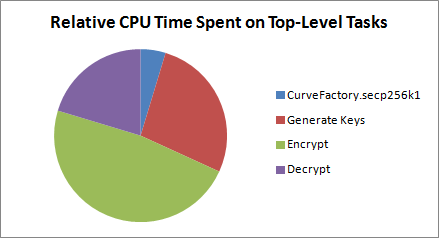
\includegraphics[width=0.70\textwidth]{performance/top-level--relative-time}
	\caption{Relative time consumption between the top level concepts: curve preparation, key generation, encryption, and decryption.}
	\label{fig:toplevel-performance}
\end{figure}

Encryption is by far the most time-consuming of the top-level operations (Figure \ref{fig:toplevel-performance}), whereas decryption and
key generation take around the same time. This is only natural, as encryption uses more iterations and more scalar multiplications.

Encoding and decoding is performed inside encryption and decryption, respectively, but both of these transformations from message to
point take a negligible amount of time. Encoding takes around \(~5\%\) of the time spent encrypting, and decoding takes around \(~0\%\)
of the time spent decrypting.

In the following is an investigation of the time spent in the application from the different abstraction levels of the architecture.
The top-most level was discussed above, and the following will look at the Point layer, the Finite Field layer, and finally at the
integer conversions that take place (a suspected bottleneck).

\subsubsection{Point Multiplication}
\label{sec:performance_components_multiplication}

All of the most time consuming top-level abstractions -- encryption, decryption and key generation -- use point multiplication.

It is an oft repeated fact that elliptic curve applications spend most of their time performing scalar point multiplication. We expect a
majority of the time being spent here, and indeed that is what we find (Figure \ref{fig:point-multiplication-performance}). \(91.2\%\) of
total computation time is spent doing point multiplications.

\begin{figure}[htb]
	\centering
	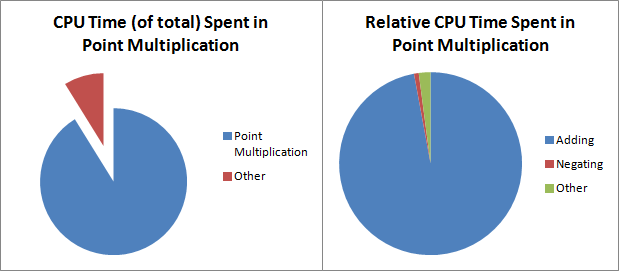
\includegraphics[width=1\textwidth]{performance/point-multiplication--relative-time}
	\caption{Fraction of total computation time spent on point multiplications (left) and the underlying operations performed in point
		multiplication (right).}
	\label{fig:point-multiplication-performance}
\end{figure}

Of the time spent in point multiplication, a vast majority is spent in addition, an almost none of the time is spent in negation. This
is to be expected, as multiplication consists mostly of additions in some form or other.

A lot of additions are being performed. One way to lower the number of additions, and hence the time spent computing multiplications, is
using a different multiplication algorithm.

An alternative would be implementing a different type of curve (such as a Montgomery curve) which allows for a greater level of precomputation
(such as with the Montgomery ladder), and hence better performance.

\subsubsection{Finite Field Operations}
\label{sec:performance_components_finitefield}

While on the point level most of the time is spent doing multiplications, the most time consuming finite field operation is division
(\(89.2\%\), see Figure \ref{fig:finite-field-performance}). Point addition for Weierstrass curves performs a single division operation
on finite field elements, which is likely the slowest operation of the addition.

\begin{figure}[htb]
	\centering
	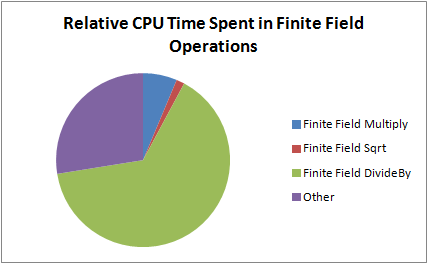
\includegraphics[width=0.6\textwidth]{performance/finite-field--relative-time}
	\caption{Time spent on finite field operations amounts to a total of \(72\%\) of total processing time. The rest of the time (notice the
		difference between point multiplication time and finite field operation time) is spent on either \texttt{BigInteger} operations or 
		general overhead.}
	\label{fig:finite-field-performance}
\end{figure}

\subsubsection{BigInteger Conversion}
\label{sec:performance_components_biginteger}

The conversion between BouncyCastle's and C\#'s native \texttt{BigInteger}s uses string conversion and parsing, which is expected to be slow.
The overall computation time spent doing just this is around \(5\%\) (see Figure \ref{fig:biginteger-performance})! Without this conversion,
the full runtime of encrypting ``Hello, World.'' would take \(466 \text{ ms}\) (\(25 \text{ ms}\) faster).

\begin{figure}[htb!]
	\centering
	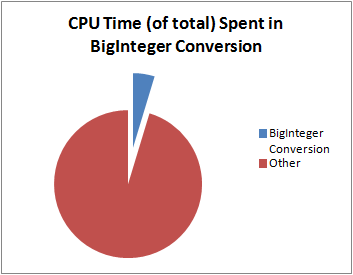
\includegraphics[width=0.6\textwidth]{performance/biginteger-conversion--relative-time}
	\caption{A decent amount of time (\(4.7\%\)) is spent on handling \texttt{BigInteger} conversions, to and from BouncyCastle's representation.
		These operations would not be required if finite field implementation using the native C\# \texttt{BigInteger}s existed.}
	\label{fig:biginteger-performance}
\end{figure}